%1.5.1
%50/50, k = 10 -> tid vs DPI!
%confusion matrix på 1 run (100, 200 og 300 DPI) 
%1.5.2
%k vs Train Size (10 runs)
%1.5.3
%cross val. 10 runs 90/10 -> mean + var


\subsection{Single Person Tests}
This section tests the KNN algorithm explained earlier using data from one single person, namely Group three member two's data.
%
%The tests are performed first with the data split equally into a 50\% for the training and 50\% for the test set and the runtime is measured and compared for the three different image qualities. 
%
%Then test are performed with changing values of k and the training set size.
%
%Afterwards with a 90/10\% split for training and test respectively is computed and mean and variance is given.
%
%All the tests will be conducted using cross validation with 10 runs.

\subsubsection{Equally Sized training and test set}
To test the algorithm the data from the three different DPI's where split 50/50\% into a training and test set. The time to compute the test set for each DPI was then recorded and plotted. This is seen in figure \ref{fig:PersonDependent_5050}.

\begin{figure}[H]
\centering
% figure...
\caption{Test result with a 50/50\% split of group three member two's data with changing . The data points are taken as the mean of 10 runs using cross validation.}
\label{fig:PersonDependent_5050}
\end{figure}

As seen on figure \ref{fig:PersonDependent_5050} then \textbf{...}.

Running the three test sets resulted in the following confusion matrices seen in table ....

\textbf{CONFUSION MATIX * 3}




\subsubsection{Changing K and Training Set Size}
Furthermore a test was performed to see how both the value of K and size of the training set affects the accuracy of the K-NN algorithm. The result is given in figure \ref{fig:personDependent_contour}.

\begin{figure}[H]
\centering
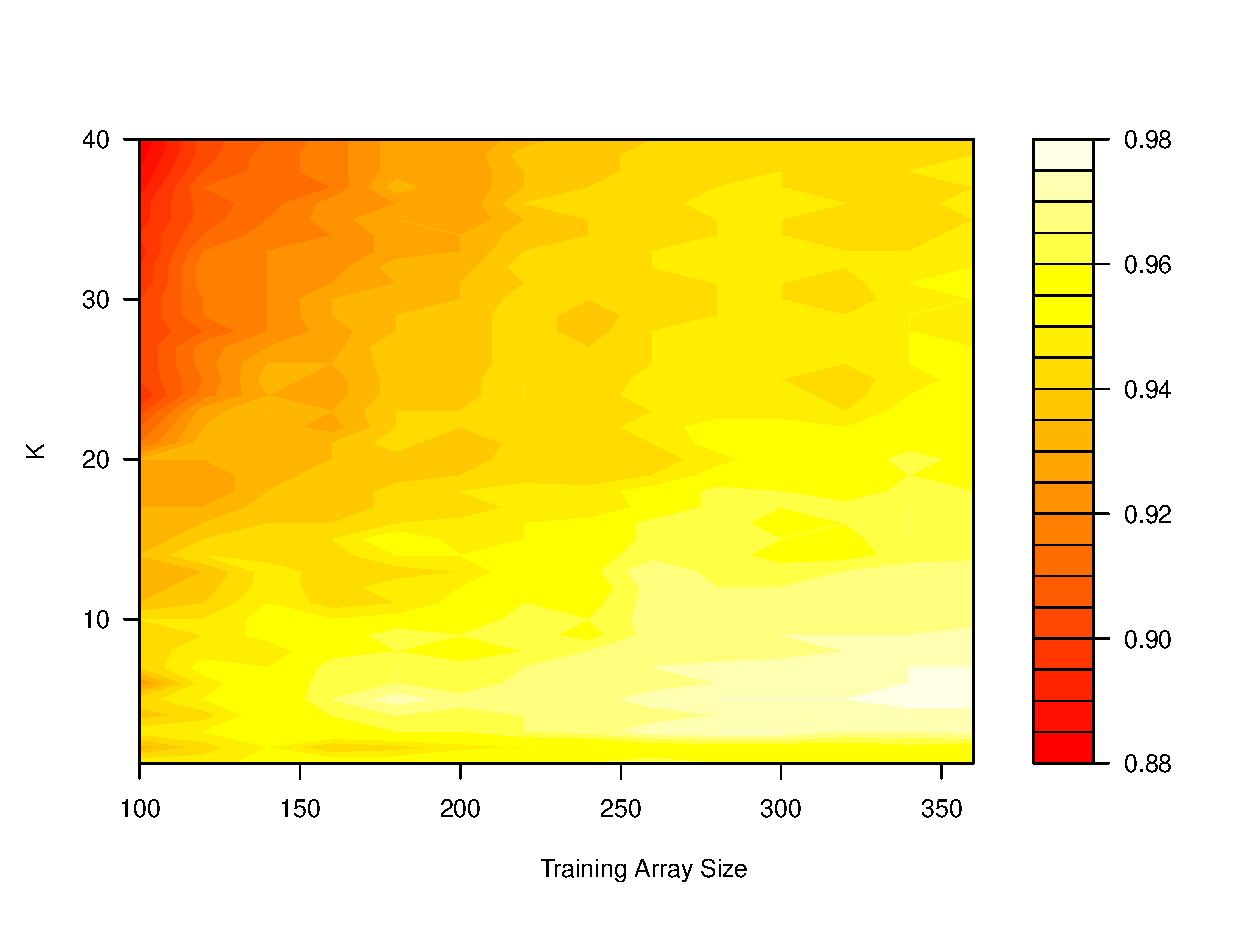
\includegraphics[width = 13cm]{graphics/graph_G3M2_20}
\caption{Success Rate of the K-NN algorithm for changing values of K and the training set size.}
\label{fig:personDependent_contour}
\end{figure}

\begin{figure}[H]
\centering
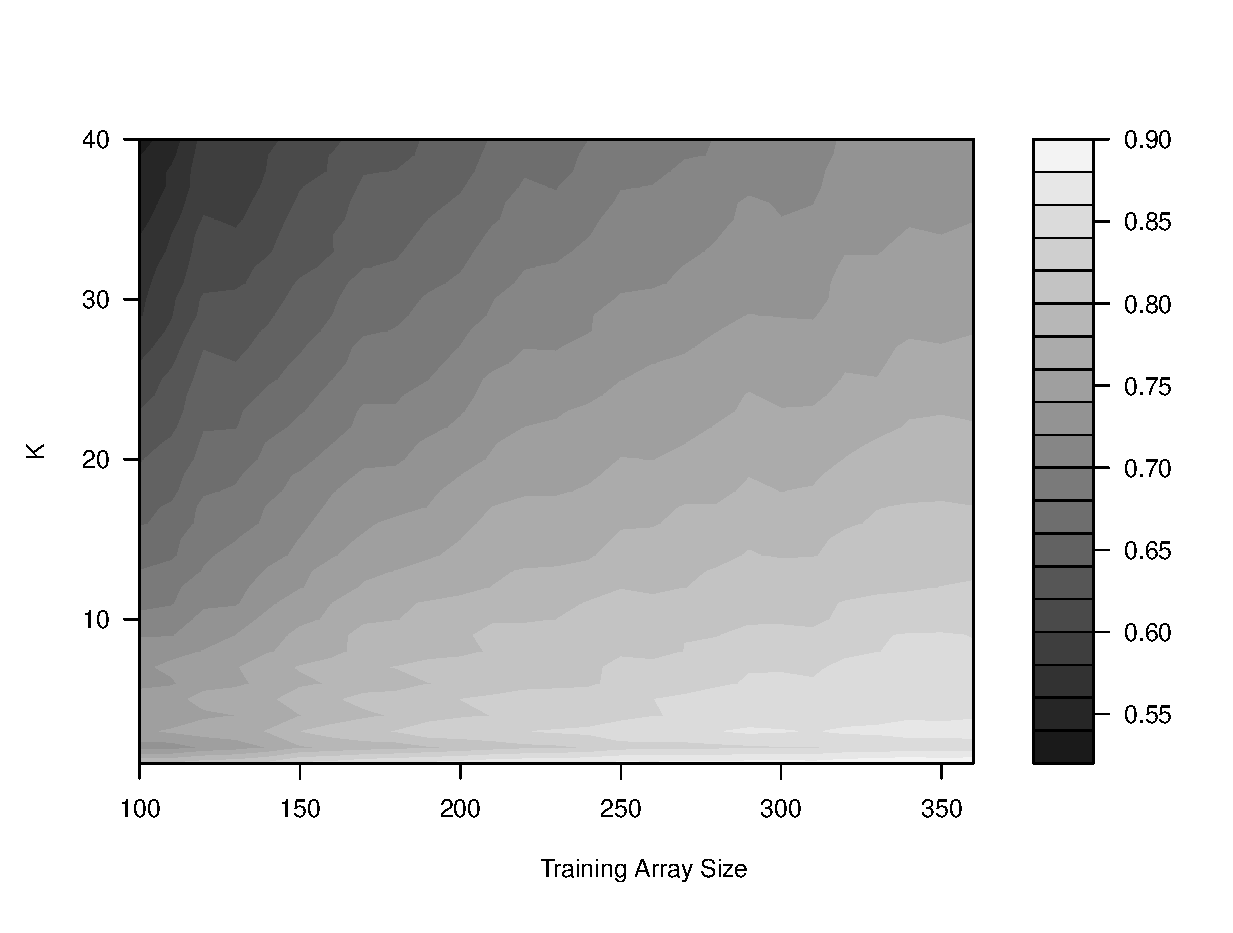
\includegraphics[width = 13cm]{graphics/graph_G3M2_10_10}
\caption{Success Rate of the K-NN algorithm for changing values of K and the training set size.}
\label{fig:personDependent_contour}
\end{figure}

\begin{figure}[H]
\centering
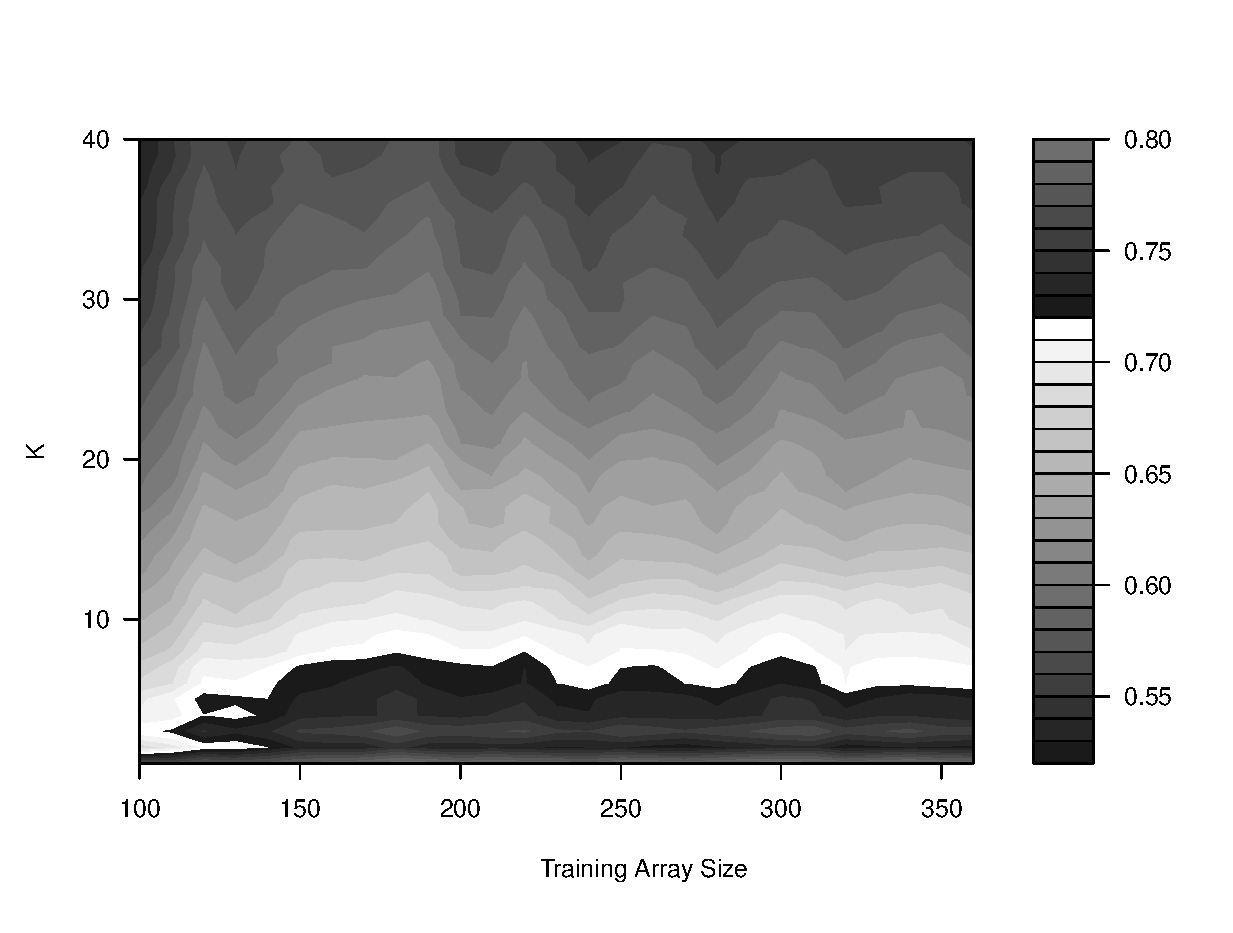
\includegraphics[width = 13cm]{graphics/graph_G3M1_10_10}
\caption{Success Rate of the K-NN algorithm for changing values of K and the training set size.}
\label{fig:personDependent_contour}
\end{figure}

The test conducted in figure \ref{fig:personDependent_contour} where done with a test size of 40 and run 10 times with cross validation.

As seen on figure \ref{fig:personDependent_contour}, then the accuracy of the algorithm appears to increase as the train set size increases.
Furthermore the optimal value of K is dependent on the size of training set. 
As the size of the training set increases, so does the area where a the best performance is obtained.
From figure \ref{fig:personDependent_contour} it can hence be seen that the results are best when using a training size which is above 300 and K ranging between 3 and 7.


\subsubsection{90/10 Data Split}
A cross validation was also carried out using a 90/10\% split of the data. 
The result of this is seen in figure \ref{fig:PersonDependent_9010}.


\begin{figure}[H]
\centering
% figure...
\caption{Test result with a 90/10\% split of group three member two's data with changing values for \textit{K}. The data points are taken as the mean of 10 runs using cross validation.}
\label{fig:PersonDependent_9010}
\end{figure}

Figure \ref{fig:PersonDependent_9010} \textbf{...}.

